\documentclass[11pt,a4paper,oneside]{report}


\usepackage{amsmath,amssymb,calc,ifthen}

\usepackage{float}
%\usepackage{cancel}

\usepackage[table,usenames,dvipsnames]{xcolor} % for coloured cells in tables

\usepackage{tikz}

% Allows us to click on links and references!

\usepackage{hyperref}
\hypersetup{
    colorlinks,
    citecolor=black,
    filecolor=black,
    linkcolor=black,
    urlcolor=black
}

% Nice package for plotting graphs
% See excellent guide:
% http://www.tug.org/TUGboat/tb31-1/tb97wright-pgfplots.pdf
\usetikzlibrary{plotmarks}
\usepackage{amsmath,graphicx}
\usepackage{epstopdf}
\usepackage{caption}
\usepackage{subcaption}

% highlight - useful for TODOs and similar
\usepackage{color}
\newcommand{\hilight}[1]{\colorbox{yellow}{#1}}

\newcommand\ci{\perp\!\!\!\perp} % perpendicular sign
\newcommand*\rfrac[2]{{}^{#1}\!/_{#2}} % diagonal fraction

\usepackage{listings}



% margin size
\usepackage[margin=1in]{geometry}

\tikzstyle{state}=[circle,thick,draw=black, align=center, minimum size=2.1cm,
inner sep=0]
\tikzstyle{vertex}=[circle,thick,draw=black]
\tikzstyle{terminal}=[rectangle,thick,draw=black]
\tikzstyle{edge} = [draw,thick]
\tikzstyle{lo} = [edge,dotted]
\tikzstyle{hi} = [edge]
\tikzstyle{trans} = [edge,->]


\definecolor{mygreen}{rgb}{0,0.6,0}
\definecolor{mygray}{rgb}{0.5,0.5,0.5}
\definecolor{mymauve}{rgb}{0.58,0,0.82}

\lstset{ %
  backgroundcolor=\color{white},   % choose the background color; you must add 
%\usepackage{color} or \usepackage{xcolor}
  basicstyle=\footnotesize,        % the size of the fonts that are used for the 
%code
  breakatwhitespace=false,         % sets if automatic breaks should only happen 
%at whitespace
  breaklines=true,                 % sets automatic line breaking
  captionpos=b,                    % sets the caption-position to bottom
  commentstyle=\color{mygreen},    % comment style
  deletekeywords={...},            % if you want to delete keywords from the 
%given language
  escapeinside={\%*}{*)},          % if you want to add LaTeX within your code
  extendedchars=true,              % lets you use non-ASCII characters; for 
%8-bits encodings only, does not work with UTF-8
  frame=single,                    % adds a frame around the code
  keepspaces=true,                 % keeps spaces in text, useful for keeping 
%indentation of code (possibly needs columns=flexible)
  keywordstyle=\color{blue},       % keyword style
  language=Octave,                 % the language of the code
  morekeywords={*,...},            % if you want to add more keywords to the set
  numbers=left,                    % where to put the line-numbers; possible 
%values are (none, left, right)
  numbersep=5pt,                   % how far the line-numbers are from the code
  numberstyle=\tiny\color{mygray}, % the style that is used for the line-numbers
  rulecolor=\color{black},         % if not set, the frame-color may be changed 
%on line-breaks within not-black text (e.g. comments (green here))
  showspaces=false,                % show spaces everywhere adding particular 
%underscores; it overrides 'showstringspaces'
  showstringspaces=false,          % underline spaces within strings only
  showtabs=false,                  % show tabs within strings adding particular 
%underscores
  stepnumber=2,                    % the step between two line-numbers. If it's 
%1, each line will be numbered
  stringstyle=\color{mymauve},     % string literal style
  tabsize=2,                       % sets default tabsize to 2 spaces
  title=\lstname                   % show the filename of files included with 
%\lstinputlisting; also try caption instead of title
}


\title{Graphical Models Coursework 1}
\author{
    Razvan Valentin Marinescu\\
    \texttt{razvan.marinescu.14@ucl.ac.uk}
    \and
    David Owen\\
    \texttt{david.owen.14@ucl.ac.uk}
    \and
    Kin Quan\\
    \texttt{kin.quan.10@ucl.ac.uk}
}

\begin{document}
\belowdisplayskip=12pt plus 3pt minus 9pt
\belowdisplayshortskip=7pt plus 3pt minus 4pt

\maketitle{}


\section*{Problem 2.5}
Define the set of nodes as $\left\{x_{1}, \ldots , x_{n} \right\}$ where $n$ is the number of nodes in DAG and the edges of DAG is defined as $\left\{ (x_{i},x_{j}) | x_{i} \rightarrow x_{j}, i \neq j \right\}$. \\
\newline
Let us find the ancestors of a node $x_{i}$.
\begin{enumerate}
	\item Look at each of the edge in the DAG, if the edge is of the form $(x_{k},x_{i})$ then go to the next step, if not then stop.
	\item Repeat the same process for every $x_{k}$ until you come to a stop.
	\item List the nodes.
\end{enumerate}
This gives a list of ancestors for $x_{i}$ in the DAG.

\section*{Problem 2.6}

The histogram is generated using the Floyd-Warshall algorithm. This finds the minimum distance between all pairs of nodes on a directed graph. In order to apply this to the Wikipedia data, the adjacency matrix is first made symmetrical (i.e. undirected), to reflect that $i$ knowing $j$ implies $j$ knows $i$, as stated in the question.


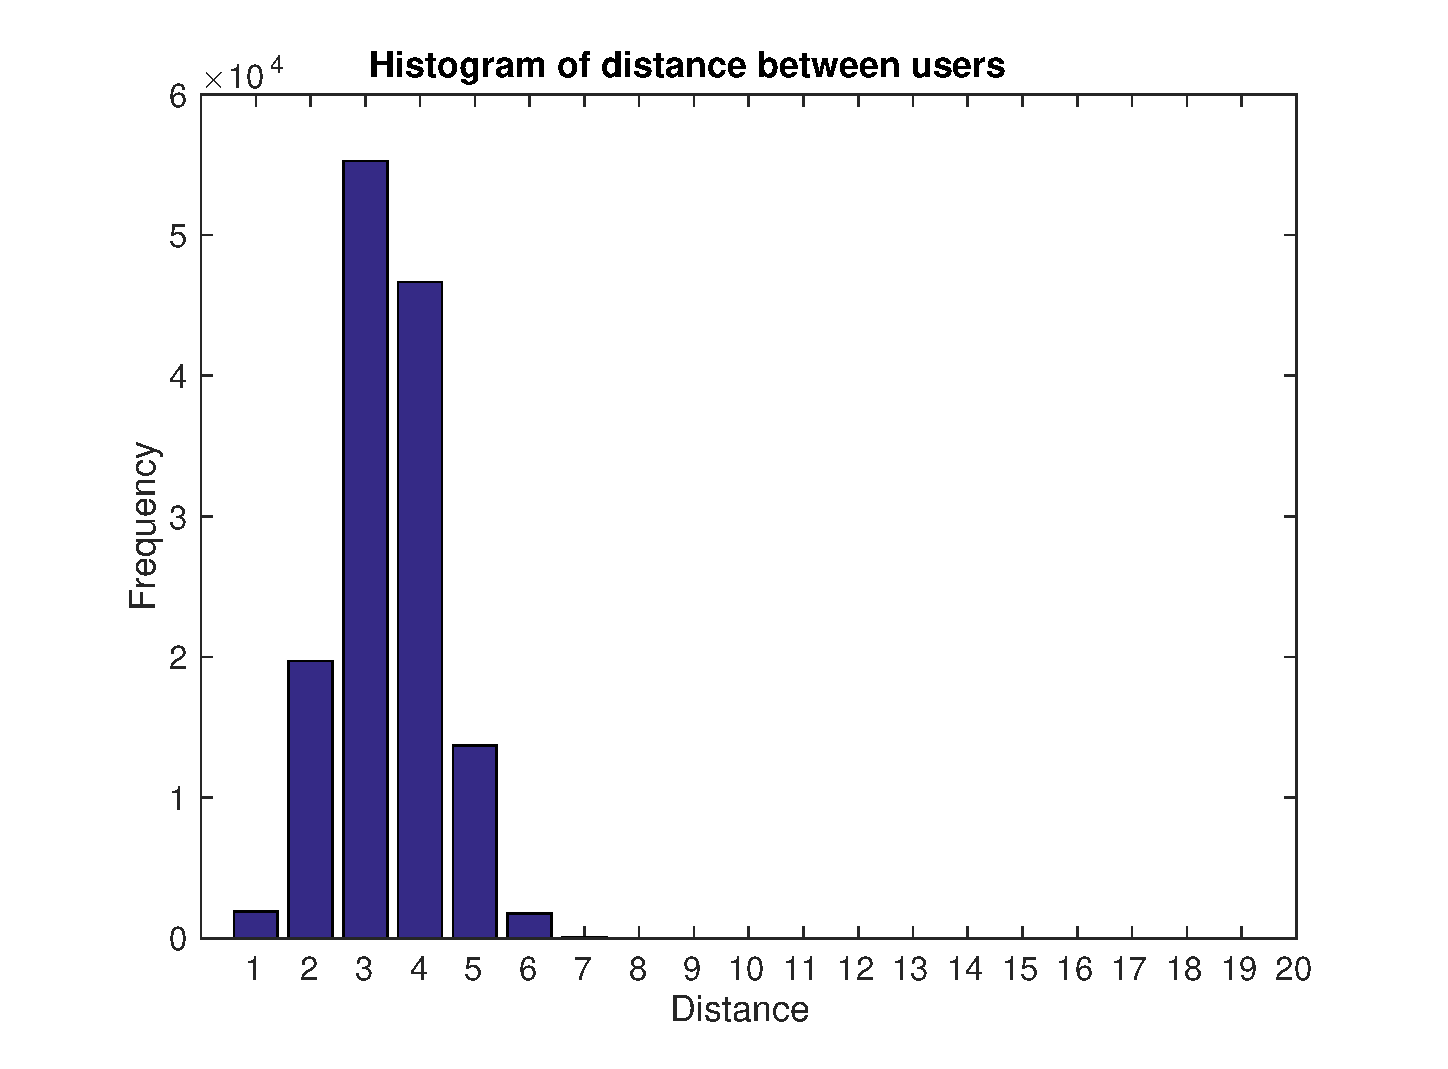
\includegraphics[scale=0.6]{plots/206_histogram}


\begin{lstlisting}
using MAT
using PyPlot

vars = matread("/Users/davido/code/BRML/data/WikiAdjSmall.mat")

# get adjacency matrix
V = vars["A"]

# make a new copy of V, which will be processed to be symmetric and [0,1]
V_new = copy(V)

# make adjacency matrix symmetric, because we assume it's undirected
for i in 1:size(V_new)[1]
        for j in 1:size(V_new)[2]
                if (V[i,j]==1) || (V[j,i]==1)
                        V_new[i,j] = 1
                        V_new[j,i] = 1
                elseif ((V[i,j]!=0) && (V[j,i]!=0))
                        println(i,",",j)
                        error("CANNOT TRANSFORM TO ADJACENCY MATRIX!")
                end
        end
end

# initialise distances matrix at Inf for every pair
dists = ones(size(V_new)) * Inf

# Floyd-Warshall loop: figure out the minimum distance from each node to every other node
for i in 1:size(dists)[1]
        dists[i,i] = 0
end

for i in 1:size(dists)[1]
        for j in 1:size(dists)[1]
                if V_new[i,j] > 0
                        dists[i,j] = V_new[i,j]
                end
        end
end

for i in 1:size(dists)[1]
        for j in 1:size(dists)[1]
                for k in 1:size(dists)[1]
                        if dists[j,k] > dists[j,i] + dists[i,k]
                                dists[j,k] = dists[j,i] + dists[i,k]
                        end
                end
        end
end

# extract relevant output -- can't just hist() whole matrix, because diagonals are irrelevant
output = Float64[]

for i in 1:size(V_new)[1]
        for j in 1:size(V_new)[2]
                if i < j
                        push!(output, dists[i,j])
                end
        end
end

h = PyPlot.plt.hist(output, 0:1:20)

\end{lstlisting}

\section*{Problem 2.7}
The algorithm shown here iterates over all cliques listed, adding them to the
cell array of maximal cliques only if they are unique and are not contained
within another clique. Cliques are then converted from a binary representation
as discussed in the question.

This yields the following list of unique maximal cliques: 119, 447, 463, 487,
703, 751, 755, 765, 831, 863, 886, 893, 954, 983, 1006.

\begin{lstlisting}
function [maxCliques] = prob27()
C = load('cliques.mat');

C = C.cl;
len = length(C);

maxCliques = cell(100,1);
count = 1
for c1=1:len
    isContained = 0;
    for c2=1:len
        if(c1 ~= c2 && all(ismember(C{c1}, C{c2})))
            isContained = isContained + 1;
            break
        end
    end
    if(isContained == 0)
       maxCliques{count} = C{c1};
       count = count + 1;
    end
end

%celldisp(maxCliques(1:count));

decCliques = zeros(count,1);
for i=1:count-1
    decCliques(i) = cliqueToDec(maxCliques{i});
end
    
sort(decCliques)
%size(maxCliques);
end
\end{lstlisting}

\begin{lstlisting}

function [dec] = cliqueToDec(clique)

%binarray = zeros(10,1);
dec = 0;
for i=1:10
    if (ismember(i, clique))
        %binarray(i) = 1
        dec = dec + 2^(10-i);
    end
end

end

\end{lstlisting}


\section*{Problem 2.9}
Let $N=3n$ where $n$ is an integer, let us prove the hypothesis by induction on $n$. Consider $n=1$ i.e. when $N=3$. This is trivial as there is three nodes with no edges therefore there are three cliques that are form. Let us now assume that the hypothesis is true for for $N$ therefore there exist a graph $G$ such that it displays all the properties stated in the question. To prove the hypothesis let us consider the graph $G$ and introduce a new partition of three nodes. For each node in the partition let us connect it to every node in $G$. Therefore the maximal cliques will contain $N-1$ edges furthermore there will only exist $3^{N/3}$ maximal cliques otherwise to form a new maximal cliques a node in $G$ would have to connect another node in the same partition. Thus for each of the three newly introduced node there would be $3^{N/3}$ maximal cliques thus the total maximal cliques is $3(3^{N/3}) = 3^{(N+1)/3}$. Thus the hypothesis is proved.

\section*{Problem 3.3}

\begin{itemize}
 \item $tuberculosis \ci smoking\;|\; shortness\;of\;breath$ is \textbf{false}, 
because path $t \to e \to d \to b \to s$ is not blocked
 \item $lung\;cancer \ci  bronchitis\;|\;smoking$ is \textbf{true}, because:
  \begin{itemize}
    \item path $l \to s \to b$ is blocked ($s$ is instantiated)
    \item path $l \to e \to d \to b$ is blocked (has collider ${e,d,b}$)
  \end{itemize}
 \item $visit \; to \; Asia \ci smoking\;|\;lung\;cancer$ is \textbf{true}, 
because:
   \begin{itemize}
    \item path $a \to t \to e \to l \to s$ is blocked ($l$ is instantiated)
    \item path $a \to t \to e \to d \to b \to s$ is blocked ($d$ is 
uninstantiated)
  \end{itemize}
 \item $visit \; to \; Asia \ci smoking\;|\;lung \; cancer; \; shortness \; of 
\; breath$ is \textbf{false} because path $a \to t \to e \to d \to b \to s$ is 
not blocked ($d$ is instantiated).
\end{itemize}



\section*{Problem 3.4}


\subsection*{1. Computation for $p(d)$}

$$p(t) = \sum_{a}p(t,a) = \sum_{a}p(t|a)p(a) = 
\begin{pmatrix}
   0.0104\\
   0.9896
\end{pmatrix}
$$

$$p(l) = \sum_{s}p(l,s) = \sum_{s}p(l|s)p(s) = 
\begin{pmatrix}
   0.055\\
   0.945
\end{pmatrix}
$$

$$p(b) = \sum_{s}p(b,s) = \sum_{s}p(b|s)p(s) = 
\begin{pmatrix}
   0.45\\
   0.55
\end{pmatrix}
$$

Given that nodes $e$ and $d$ are not instantiated, we get that $t \ci l$ and $e 
\ci b$, which implies that $p(t,l) = p(t)p(l)$ and $p(e,b)=p(e)p(b)$. We can 
now calculate:

$$p(e) = \sum_{t,l}p(e,t,l) = \sum_{t,l}p(e|t,l)p(t,l) = 
\sum_{t,l}p(e|t,l)p(t)p(l) = 
\begin{pmatrix}
   0.0648\\
   0.9351
\end{pmatrix}
$$

$$p(d) = \sum_{e,b}p(d,e,b) = \sum_{e,b}p(d|e,b)p(e,b) = 
\sum_{e,b}p(d|e,b)p(e)p(b) = 
\begin{pmatrix}
   0.4359\\
   0.5640
\end{pmatrix}
$$
 
% julia> pE = sum(pAll, [A T B X S D L])
% PotArray([7],[0.06482800000000001,0.935172])
% 
% julia> pX = sum(pAll, [A T E B S D L])
% PotArray([5],[0.11029004000000005,0.88970996])
% 
% julia> pD = sum(pAll, [A T E B X S L])
% PotArray([6],[0.4359706000000001,0.5640293999999999])

\subsection*{2. Computation for $p(d|s = tr)$}

We can calculate $p(d| s = tr$ by re-doing the same calculations as 
before, but this time setting the prior probability of s to $p(s) = 
\begin{pmatrix}
                                                              1\\
                                                              0
                                                             \end{pmatrix}$. 
Moreover, we don't need to recalculate $p(t)$ because its probability remains 
unchanged.

$$p(l) = \sum_{s}p(l,s) = \sum_{s}p(l|s)p(s) = 
\begin{pmatrix}
   0.1\\
   0.9
\end{pmatrix}
$$

$$p(b) = \sum_{s}p(b,s) = \sum_{s}p(b|s)p(s) = 
\begin{pmatrix}
   0.6\\
   0.4
\end{pmatrix}
$$

Given that nodes $e$ and $d$ are not instantiated, we get that $t \ci l$ and $e 
\ci b$, which implies that $p(t,l) = p(t)p(l)$ and $p(e,b)=p(e)p(b)$. We can 
now calculate:

$$p(e) = \sum_{t,l}p(e,t,l) = \sum_{t,l}p(e|t,l)p(t,l) = 
\sum_{t,l}p(e|t,l)p(t)p(l) = 
\begin{pmatrix}
   0.1093\\
   0.8906
\end{pmatrix}
$$

$$p(d) = \sum_{e,b}p(d,e,b) = \sum_{e,b}p(d|e,b)p(e,b) = 
\sum_{e,b}p(d|e,b)p(e)p(b) = 
\begin{pmatrix}
   0.5528\\
   0.4471
\end{pmatrix}
$$



\subsection*{3. Computation for $p(d|s = fa)$}

We adopt a similar strategy for $p(d| s = fa$ We set $p(s) = \begin{pmatrix}
                                                              0\\
                                                              1
                                                             \end{pmatrix}$ and 
we get:

$$p(l) = \sum_{s}p(l,s) = \sum_{s}p(l|s)p(s) = 
\begin{pmatrix}
   0.01\\
   0.99
\end{pmatrix}
$$

$$p(b) = \sum_{s}p(b,s) = \sum_{s}p(b|s)p(s) = 
\begin{pmatrix}
   0.3\\
   0.7
\end{pmatrix}
$$

Given that nodes $e$ and $d$ are not instantiated, we get that $t \ci l$ and $e 
\ci b$, which implies that $p(t,l) = p(t)p(l)$ and $p(e,b)=p(e)p(b)$. We can 
now calculate:

$$p(e) = \sum_{t,l}p(e,t,l) = \sum_{t,l}p(e|t,l)p(t,l) = 
\sum_{t,l}p(e|t,l)p(t)p(l) = 
\begin{pmatrix}
   0.0202\\
   0.9797
\end{pmatrix}
$$

$$p(d) = \sum_{e,b}p(d,e,b) = \sum_{e,b}p(d|e,b)p(e,b) = 
\sum_{e,b}p(d|e,b)p(e)p(b) = 
\begin{pmatrix}
   0.3191\\
   0.6808
\end{pmatrix}
$$


\section*{Problem 3.8}
\begin{enumerate}
	\item 
	\begin{enumerate}
		\item Let us find $p(B=tr|W=tr)$, by Bayes' rule:
		\begin{align}
		p(B=tr|W=tr) &= \frac{p(B = tr , W = tr)}{p(W =tr)} \\
		&= \frac{p(W = tr | B = tr)p(B = tr)}{p(W=tr)} \\
		&= \frac{p(W = tr | B = tr)p(B = tr)}{\sum_{A, B}~p(W = tr| A)p(A|B)}\\		
		\end{align}
	To find $p(W = tr | B = tr)$ lets us use Bayes' rule again:
	\begin{align}
	p(W = tr | B = tr) &= \sum_{A} p(A|B=tr)p(W = tr|A)\\
	&= 0.99\times0.9+(1-0.99)\times0.5\\
	&= 0.896.
	\end{align}
	Combining the results from above gives:
	\begin{align}
	p(B=tr|W=tr) &= \frac{0.896\times0.01}{0.01\times(0.99\times0.9+0.01\times 0.5)+0.99(0.05\times 0.9 + 0.95\times 0.5)}\\
	&= 0.0171.
	\end{align}
	\item
	Lets find $p(B=tr|W=tr,G=fa)$, by Bayes' rule:
	\begin{equation}
	p(B=tr|W=tr,G=fa) = \frac{p(W=tr, G=fa | A)\times p(B=tr)}{p(W=tr, G=fa)}
	\end{equation}
	Let us find $p(W=tr, G=fa | A)$,
	\begin{align}
	p(W=tr, G=fa | A) &= \sum_{A} p(W=tr, G=fa |A)p(A|B=tr)\\
	&=0.9 \times 0.3 \times 0.99+ 0.5\times 0.8 \times 0.01\\
	&= 0.2713
	\end{align}
	Combining the results from above gives:
	\begin{align}
	p(B=tr|W=tr,G=fa) &= \frac{0.2713 \times 0.01}{\sum_{A,B}~p(W=tr |A) p(G=fa|A) p(A|B)}\\
	&= {0.002713}\times(0.01\times (0.99 \times 0.9 \times 0.3 + 0.01 \times 0.5 \times 0.8) \nonumber \\
	&+0.99\times(0.05 \times 0.9 \times 0.3 + 0.95 \times 0.9 \times 0.8))^{-1}\\
	&= 0.004.
	\end{align}
	\end{enumerate}
	\item Since $\tilde{G} = fa$ then $p(G=fa) = 0.9$ and  $p(G=tr) = 0.1$. Also since $\tilde{W} = tr$ then $p(W=fa) = 0.7$ and $p(W=tr)=0.3$.
	\begin{enumerate}
		\item Let us find $p(B=tr | \tilde{W})$.
		\begin{equation}
		p(B=tr | \tilde{W}) = \sum_{W} p(B= tr|W)p(W |\tilde{W})
		\end{equation}
		In order to compute the above, let us first compute $p(B=tr|W=fa)$. By Bayes' law:
		\begin{align}
		p(B=tr|W=fa) &= \frac{p(W=fa|B=tr)p(B=tr)}{p(W=fa)}\\
		&= \frac{(1-0.896)\times 0.01}{1-0.523}\\
		&= 0.002.
		\end{align}
		Thus from above
		\begin{align}
		p(B=tr | \tilde{W}) &= 0.3\times 0.017 + 0.7 \times 0.002\\
		&=0.007
		\end{align}
		\item
		Let us find $p(B=tr|\tilde{W},\tilde{G})$, since $W$ and $G$ are independent then
		\begin{equation}
		p(B=tr|\tilde{W},\tilde{G}) = \sum_{W,G} {p(B=tr|W,G) p(W|\tilde{W}) p(G|\tilde{G})}.
		\end{equation}
		By Bayes' rule;
		\begin{equation}
		p(B=tr|\tilde{W},\tilde{G}) = \sum_{W,G} \frac{p(W,G|B=tr) p(B=tr) p(W|\tilde{W}) p(G|\tilde{G})}{p(W,G)}.
		\end{equation}
		In order to compute the above, we require to compute the following:
		\begin{enumerate}
			\item
			\begin{align}
			p(W=tr, G=tr|B=tr) &= p(W=tr|B=tr)p(G=tr|B=tr),\\
			&= \sum_{A} p(W=tr, A|B=tr) p(G=tr, A|B=tr),\\
			&= 0.99 \times 0.9 \times 0.7 + 0.01 \times 0.5 \times 0.2,\\
			&= 0.625.
			\end{align}
			\item
			\begin{align}
			p(W=fa, G=tr|B=tr) &= p(W=fa|B=tr)p(G=tr|B=tr),\\
			&= \sum_{A} p(W=fa, A|B=tr) p(G=tr, A|B=tr),\\
			&= 0.99 \times 0.1 \times 0.7 + 0.01 \times 0.5 \times 0.2\\
			&= 0.070.
			\end{align}
			\item
			\begin{align}
			p(W=fa,G=fa|B=tr)&= p(W=fa|B=tr) p(G=fa|B=tr)\\
			&= \sum_{A} p(W=fa, A|B=tr) p(G=fa, A|B=tr),\\
			&= 0.99\times 0.1 \times 0.3 + 0.01 \times 0.5 \times 0.8,\\
			&= 0.034.
			\end{align}
			\item
			\begin{align}
			p(W=tr,G=fa|B=tr)&= p(W=tr|B=tr) p(G=fa|B=tr)\\
			&= \sum_{A} p(W=tr, A|B=tr) p(G=fa, A|B=tr),\\
			&= 0.99 \times 0.9 \times 0.3 + 0.01 \times 0.5 \times 0.8,\\
			&= 0.271
			\end{align}
			\item
			\begin{align}
			p(W=tr,G=tr)&=\sum_{B} p(W=tr,G=tr|B)p(B) \\
			&=0.131
			\end{align}
			\item
			\begin{align}
			p(W=tr,G=fa)&=\sum_{B} p(W=tr,G=fa|B)p(B) \\
			&= 0.380
			\end{align}
			\item
			\begin{align}
			p(W=fa,G=tr)&= \sum_{B} p(W=tr,G=fa|B)p(B)\\
			&=0.098.
			\end{align}
			\item
			\begin{align}
			p(W=fa,G=fa)&= \sum_{B} p(W=fa, G=fa|B)p(B) \\
			&=0.378.
			\end{align}
		\end{enumerate}
		Hence using all the above gives:
		\begin{align}
		p(B=tr|\tilde{W},\tilde{G}) = 0.031
		\end{align}
	\end{enumerate}
\end{enumerate}

\section*{Problem 3.9}

\subsection*{1. Belief network}

\begin{figure}[H]
  \centering
    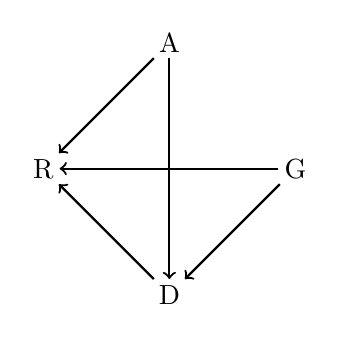
\begin{tikzpicture}[scale=0.8,help lines/.style={color=lightgray,line 
width=0.2pt},post/.style={->,shorten >=1pt,>=stealth',thick}]
    
    \node[inner sep=2] (A) at (0.0,2.0){A};
    \node[inner sep=2] (G) at (2.0,0.0) {G};
    \node[inner sep=2] (R) at (-2.0,0.0) {R};
    \node[inner sep=2] (D) at (0.0,-2.0) {D};

    \draw[->, thick] (A) -- (R);
    \draw[->, thick] (A) -- (D);
    \draw[->, thick] (G) -- (D);
    \draw[->, thick] (G) -- (R);
    \draw[->, thick] (D) -- (R);
    
    \end{tikzpicture}
    \caption{Belief network}
    \label{fig:all_trade_cca_black}     
\end{figure}

\subsection*{2. Computation of $p(R=tr \; | \; D=tr)$}

By considering the generative model and marginalising we get 
\begin{equation}
p(R=tr \; | \; D=tr) = \sum\limits_{A,G} p(R=tr \;
| A, \; G,\; D=tr) p(A) p(G) p(D=tr \; | \; G, \; A)
\end{equation}

This suggests that from a database of patient entries we 
take the number of patients who received the drug \emph{and} recovered, and
then divide it by the total number of patients who received the drug. 

\subsection*{3. Computation of $p(recover \; | \; do(drug),\; young)$}

The do-calculus allows us to deal with interventional studies, in which we
have specifically \emph{set} a causal condition in the experiment. The causal
variable (here $D$) is set to its interventional value, and then severed from
its parent variables. This yields the following new DAG:


\begin{figure}[H]
  \centering
    \begin{tikzpicture}[scale=0.8,help lines/.style={color=lightgray,line 
width=0.2pt},post/.style={->,shorten >=1pt,>=stealth',thick}]
    
    \node[inner sep=2] (A) at (0.0,2.0){A};
    \node[inner sep=2] (G) at (2.0,0.0) {G};
    \node[inner sep=2] (R) at (-2.0,0.0) {R};
    \node[inner sep=2] (D) at (0.0,-2.0) {D};

    \draw[->, thick] (A) -- (R);
    \draw[->, thick] (G) -- (R);
    \draw[->, thick] (D) -- (R);
    
    \end{tikzpicture}
    \caption{Belief network}
    \label{fig:do_calc_DAG}    
\end{figure}

Hence, from the generative model
\begin{equation}
p(R=tr \; | \; do(drug),\; A=yo) =
\sum\limits_{G} p(R=tr \; | \; do(drug), \; A=yo, \; G) p(G)
\end{equation}

To calculate this, we must take the target group (young people) and then examine their
recovery results by gender. We then produce a weighted sum of their recovery
probability, weighted by the proportions of each gender in the study. 

%\hilight{David, could you please write the answer for this one?}

\section*{Problem 3.11}

In order to include this effect in our model, we change the formula for the 
joint probability distribution to be:

$$p(B, E, A, R) = p(A|B, E)p(R|E)p(B|E)p(E)$$

This means that on the graphical model we add an arrow from $E$ to $B$. The 
belief network diagram will look like this:

\begin{figure}[H]
  \centering
    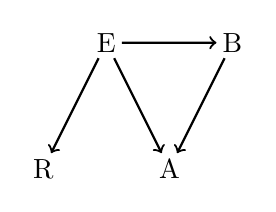
\begin{tikzpicture}[scale=0.8,help lines/.style={color=lightgray,line 
width=0.2pt},post/.style={->,shorten >=1pt,>=stealth',thick}]
    
    \node[inner sep=2] (E) at (0.0,2.0){E};
    \node[inner sep=2] (B) at (2.0,2.0) {B};
    \node[inner sep=2] (R) at (-1.0,0.0) {R};
    \node[inner sep=2] (A) at (1.0,0.0) {A};

    \draw[->, thick] (E) -- (B);
    \draw[->, thick] (E) -- (A);
    \draw[->, thick] (B) -- (A);
    \draw[->, thick] (E) -- (R);
    
    \end{tikzpicture}
    \caption{Belief network}
    \label{fig:all_trade_cca_black}     
\end{figure}

\section*{Problem 3.12}
Two belief networks are Markov equivalent if they represent the same conditional
independence statements. Markov equivalence between two graphs can be determined
by calculating the graphs' \emph{skeletons} and \emph{immoralities}. If they
have the same skeleton and immoralities, the two graphs are Markov equivalent.

\begin{lstlisting}
function MarkovEquiv(A, B)
    # test skeleton
    skel_A = get_skeleton(A)
    skel_B = get_skeleton(B)

    # test immoralities
    imm_A = get_immoralities(A)
    imm_B = get_immoralities(B)

    if (skel_A==skel_B) && (imm_A==imm_B)
        return true
    else
        return false
    end
end

function get_skeleton(M)
    skel = zeros(size(M))

    for i in 1:size(M)[1]
        for j in 1:size(M)[2]
            if M[i,j] == 1
                # skeleton is undirected version of the DAG
                skel[i,j] = 1
                skel[j,i] = 1
            end
        end
    end

    return skel
end

function get_immoralities(M)
    imms = Array[]
    for i in 1:size(M)[1]
        for j in 1:size(M)[2]
            for k in 1:size(M)[1]
                # if two nodes share a child but are not directly connected, they form an immorality
                if  M[i,j] == 1 && M[k,j] == 1 &&
                    M[i,k] != 1 && M[k,i] != 1 && 
                    i != j && i != k && j != k
                        push!(imms, [i, j, k])
                end
            end
        end
    end

    # sort immoralities so identical immoralities can be removed, leaving only unique immoralities
    unique_imms = unique(map(x -> sort(x), imms))

    return unique_imms
end
\end{lstlisting}


\section*{Problem 3.13}
The skeletons are equivalently:

\begin{equation}
\begin{pmatrix}
 0 & 0 & 1 & 1 & 0 & 1 & 0 & 0 & 0 \\
 0 & 0 & 1 & 0 & 1 & 0 & 0 & 0 & 0 \\
 1 & 1 & 0 & 0 & 1 & 0 & 1 & 0 & 0 \\
 1 & 0 & 0 & 0 & 0 & 1 & 0 & 1 & 1 \\
 0 & 1 & 1 & 0 & 0 & 0 & 1 & 0 & 0 \\
 1 & 0 & 0 & 1 & 0 & 0 & 0 & 1 & 0 \\
 0 & 0 & 1 & 0 & 1 & 0 & 0 & 0 & 1 \\
 0 & 0 & 0 & 1 & 0 & 1 & 0 & 0 & 0 \\
 0 & 0 & 0 & 1 & 0 & 0 & 1 & 0 & 0 \\
\end{pmatrix}
\end{equation}

The immoralities are equivalently $\left( 1, 2, 3\right)$, $\left( 1, 3, 5 \right)$ and
$\left( 4, 7, 9 \right)$.

Hence the two graphs are Markov equivalent.

\section*{Problem 3.14}
By considering conditional probabilities and evidence at the parent nodes, and 
then calculating the marginals over these, the \emph{a posteriori} probability 
vector can be computed.

\hilight{Raz probably wants to expand on this.}

\begin{equation}
\begin{split}
\begin{bmatrix}
p(C_{12} = 1 \; | \; C) \; , \; p(C_{13} = 1 \; | \; C)  \; , \; p(C_{23} = 1 \; | \; C) \; , \; p(C_{32} = 1 \; | \; C) \; , \;
p(C_{21} = 1 \; | \; C) \; , \; p(C_{31} = 1 \; | \; C) 
\end{bmatrix} \\ = 
\begin{bmatrix}
0.9174 \; , \; 0.1597 \; , \; 0 \; , \; 0.1743 \; , \; 0.1 \; , \; 0.0850
\end{bmatrix}
\end{split}
\end{equation}

\begin{lstlisting}

function [] = prob314()

%c122, c232, c121323, c232113 = 1,2,3,4

%indexC12 = PotArray(c121323, [0 0 0 0 1 1 1 1])
initProb = [0.9 0.1];
pC12 = initProb;
pC13 = initProb;
pC23 = initProb;
pC32 = initProb;
pC31 = initProb;
pC21 = initProb;

pC121332 = [0.9^3 0.9^2*0.1 0.9^2*0.1 0.9*0.1^2 0.9^2*0.1 0.9*0.1^2 0.9*0.1^2 0.1^3];

% conditional prob tables: p(C12(2) = 1 | C12 C13 C23) and the other one
pC122gC121332 = [1 1 1 0 0 0 0 0; 0 0 0 1 1 1 1 1];
pC232gC232113 = [1 1 1 0 0 0 0 0; 0 0 0 1 1 1 1 1];

% child node states
pC122 = [0 1];
pC232 = [1 0];

% lambda messages
lamC122 = pC122 * pC122gC121332;
lamC232 = pC232 * pC232gC232113;

% calculate the lambda evidence at the parent node
p1C121332 = lamC122 .* pC121332;

% normalise the probability of the joint state
p1C121332 = p1C121332 ./ sum(p1C121332);

indicesC13 = [1,2,5,6; 3,4,7,8];
indicesC32 = [1,3,5,7; 2,4,6,8];

% calculate the marginals p(C12) p(C13) p(C23)
pC12 = [sum(p1C121332(1:4)) sum(p1C121332(5:8))];
pC13 = [sum(p1C121332(indicesC13(1,:))) sum(p1C121332(indicesC13(2,:)))];
pC32 = [sum(p1C121332(indicesC32(1,:))) sum(p1C121332(indicesC32(2,:)))];

pC232113 = [pC23(1)*pC21(1)*pC13(1) pC23(1)*pC21(1)*pC13(2) pC23(1)*pC21(2)*pC13(1) pC23(1)*pC21(2)*pC13(2) pC23(2)*pC21(1)*pC13(1) pC23(2)*pC21(1)*pC13(2) pC23(2)*pC21(2)*pC13(1) pC23(2)*pC21(2)*pC13(2)];

% calculate the lambda evidence at the parent node
p1C232113 = lamC232 .* pC232113;

% normalise the probability of the joint state
p1C232113 = p1C232113 ./ sum(p1C232113);
     
% calculate the marginals p(C23) p(C21) p(C13)
pC23 = [sum(p1C232113(1:4)) sum(p1C232113(5:8))];
pC21 = [sum(p1C232113(indicesC13(1,:))) sum(p1C232113(indicesC13(2,:)))];
pC13 = [sum(p1C232113(indicesC32(1,:))) sum(p1C232113(indicesC32(2,:)))];

display('--------------------')

pC12
pC13
pC23
pC32
pC31
pC21

        
end
\end{lstlisting}

\section*{Problem 3.15}

\subsection*{1.}
\begin{figure}[H]
  \centering
    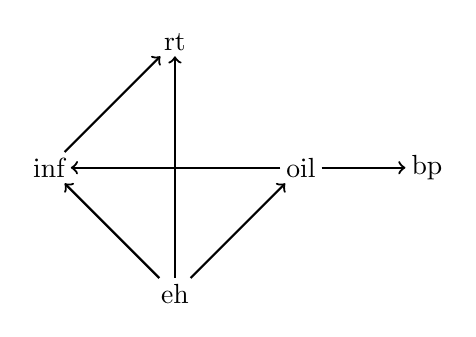
\begin{tikzpicture}[scale=0.8,help lines/.style={color=lightgray,line 
width=0.2pt},post/.style={->,shorten >=1pt,>=stealth',thick}]
    
    \node[inner sep=2] (eh) at (0.0,-2.0){eh};
    \node[inner sep=2] (oil) at (2.0,0.0) {oil};
    \node[inner sep=2] (bp) at (4.0,0.0) {bp};
    \node[inner sep=2] (inf) at (-2.0,0.0) {inf};
		\node[inner sep=2] (rt) at (0.0,2.0) {rt};

    \draw[->, thick] (oil) -- (bp);
    \draw[->, thick] (eh) -- (oil);
    \draw[->, thick] (eh) -- (inf);
    \draw[->, thick] (oil) -- (inf);
    \draw[->, thick] (eh) -- (rt);
		\draw[->, thick] (inf) -- (rt);
    
    \end{tikzpicture}
    \caption{Belief network}
    \label{fig:all_trade_cca_black}     
\end{figure}


\subsection*{2.}

The answer can be easily calculated using Julia. We first define the 
conditional probability tables and then we compute the joint distribution 
$p(eh, oil, inf, bp, rt)$. From this we calculate the marginals $p(inf,rt,bp) 
= \sum_{oil, eh}p(eh, oil, inf, bp, rt)$ and $p(rt,bp) = 
\sum_{inf}p(inf, rt, bp)$. Using these marginals we use Bayes' rule to compute 
the posterior $p(inf|rt, bp) = p(inf, rt, bp)/p(rt, bp)$. The Julia code that 
was used to compute this is given below. The final answer $p(inf = high | rt 
= high, bp = normal) = 0.984746 $\\

\begin{lstlisting}
low, high, normal = 1,2,3
E,O,I,R,B = 1,2,3,4,5

pE = PotArray(E, [2//10 8//10])
pOgE = PotArray([O E], [9//10 5//100; 1//10 95//100])


tabIgOE=zeros(2,2,2)
tabIgOE[low, low, low]=9//10
tabIgOE[low, low, high]=1//10
tabIgOE[low, high, low]=1//10
tabIgOE[low, high, high]=1//100

tabIgOE[high, low, low]=1//10
tabIgOE[high, low, high]=9//10
tabIgOE[high, high, low]=9//10
tabIgOE[high, high, high]=99//100

pIgOE = PotArray([I O E], tabIgOE)


tabRgIE=zeros(2,2,2)
tabRgIE[:, low, low]=[9//10; 1//10]
tabRgIE[:, low, high]=[1//10; 9//10]
tabRgIE[:, high, low]=[1//10; 9//10]
tabRgIE[:, high, high]=[1//100; 99//100]

pRgIE = PotArray([R I E], tabRgIE)


pBgO = PotArray([B O], [9//10 1//10; 1//10 4//10; 0//10 5//10])

pAll = pBgO * pRgIE * pIgOE * pOgE * pE

pIRB = sum(pAll, [O E])

pRB = sum(pIBR, I)

pIgRB = pIBR / pRB

\end{lstlisting}


\section*{Problem 3.17}

\subsection*{1.}

In order to prove $a \ci c$ we need to show that $p(a,c) = p(a)p(c)$. We first 
calculate the joint probability distribution $p(a,b,c) = p(c|b)p(b|a)p(a)$. 
Then 
we marginalise over $b$ to get $p(a,c)=\sum_{b} p(a,b,c) = \sum_{b} 
p(c|b)p(b|a)p(a)$. 

We will now calculate the three terms from the sum $\sum_{b} 
p(c|b)p(b|a)p(a)$. For $b=1$ we get 

% b = 1

\begin{equation}
\label{317A}
p(b = 1|a) =  
  \begin{pmatrix}
   \ 1/4 \\[0.4em]
   \ 15/40 \\
 \end{pmatrix}
\end{equation}

 
\begin{equation}
\label{317B}
    p(b = 1, a) = p(b = 1|a) p(a) = \begin{pmatrix}
      \ 3/20 \\[0.4em]
      \ 3/20 \\
    \end{pmatrix}
\end{equation}

\begin{equation}
\label{317C}
p(c | b = 1) =  
  \begin{pmatrix}
   \ 1/3 \\[0.4em]
   \ 2/3 \\
 \end{pmatrix} 
\end{equation}

Combining equations \eqref{317B} and \eqref{317C} we get:

\begin{equation}
\label{317D}
p(a, b = 1, c) =  p(c | b = 1 )p(b = 1,a)
  \begin{pmatrix}
   \ \frac{3}{20} \frac{1}{3} & \frac{3}{20} \frac{2}{3} \\[0.4em]
   \ \frac{3}{20} \frac{1}{3} & \frac{3}{20} \frac{2}{3} \\
 \end{pmatrix} = \frac{1}{40}
  \begin{pmatrix}
   \ 2 & 4 \\[0.4em]
   \ 2 & 4 \\
 \end{pmatrix} 
\end{equation}

A similar computaiton is done for $p(a, b = 2, c)$ and $p(a, b = 3, c)$. 

% b =2

\begin{equation}
\label{317E}
    p(b = 2, a) = p(b = 2|a) p(a) = 
    \begin{pmatrix}
      \ \frac{1}{12} \frac{3}{5} \\[0.4em]
      \ \frac{1}{8} \frac{2}{5} \\
    \end{pmatrix} = 
    \begin{pmatrix}
      \ 1/20 \\[0.4em]
      \ 1/20 \\
    \end{pmatrix}
\end{equation}

\begin{equation}
\label{317F}
p(c | b = 2) =  
  \begin{pmatrix}
   \ 1/2 \\[0.4em]
   \ 1/2 \\
 \end{pmatrix} 
\end{equation}

Combining equations \eqref{317E} and \eqref{317F} we get:

\begin{equation}
\label{317G}
p(a, b = 2, c) =  
  \begin{pmatrix}
   \ \frac{1}{20} \frac{1}{2} & \frac{1}{20} \frac{1}{2} \\[0.4em]
   \ \frac{1}{20} \frac{1}{2} & \frac{1}{20} \frac{1}{2} \\
 \end{pmatrix} = \frac{1}{40}
  \begin{pmatrix}
   \ 1 & 1 \\[0.4em]
   \ 1 & 1 \\
 \end{pmatrix} 
\end{equation}

%% b = 3

Now for $b = 3$ we get:

\begin{equation}
\label{317H}
    p(b = 3, a) = p(b = 3|a) p(a) = 
    \begin{pmatrix}
      \ \frac{2}{3} \frac{3}{5} \\[0.4em]
      \ \frac{1}{2} \frac{2}{5} \\
    \end{pmatrix} = \frac{1}{5}
    \begin{pmatrix}
      \ 2 \\[0.4em]
      \ 1 \\
    \end{pmatrix}
\end{equation}

\begin{equation}
\label{317I}
p(c | b = 3) =  
  \begin{pmatrix}
   \ 15/40 \\[0.4em]
   \ 5/8 \\
 \end{pmatrix} 
\end{equation}

Combining equations \eqref{317H} and \eqref{317I} we get:

\begin{equation}
\label{317J}
p(a, b = 3, c) =  
  \begin{pmatrix}
   \ \frac{2}{5} \frac{15}{40} & \frac{2}{5} \frac{5}{8} \\[0.4em]
   \ \frac{1}{5} \frac{15}{40} & \frac{1}{5} \frac{5}{8} \\
 \end{pmatrix} = \frac{1}{40}
  \begin{pmatrix}
   \ 6 & 10 \\[0.4em]
   \ 3 & 5 \\
 \end{pmatrix} 
\end{equation}

Summing up all the right-hand side terms from equations \eqref{317D},  
\eqref{317G} and  \eqref{317J} we get

\begin{equation}
\label{317K}
p(a, c) =  \sum_{b} p(a,b,c) = \frac{1}{40}
  \begin{pmatrix}
   \ 9 & 15 \\[0.4em]
   \ 6 & 10 \\
 \end{pmatrix} 
\end{equation}
 
From the joint distribution $p(a,c)$ we can calculate the marginalise

\begin{equation}
\label{317L}
p(c) =  \sum_{a} p(a,c) = \frac{1}{8}
  \begin{pmatrix}
   \ 3 \\[0.4em]
   \ 5 \\
 \end{pmatrix} 
\end{equation}
 
Using the given distribution $p(a)$ and the above equation we can now calculate:
\begin{equation}
\label{317M}
p(a)p(c) =
  \begin{pmatrix}
   \ \frac{3}{5} \frac{3}{8} & \frac{3}{5} \frac{5}{8} \\[0.4em]
   \ \frac{2}{5} \frac{3}{8} & \frac{2}{5} \frac{5}{8} \\
 \end{pmatrix} = \frac{1}{40}
  \begin{pmatrix}
   \ 9 & 15 \\[0.4em]
   \ 6 & 10 \\
 \end{pmatrix} 
\end{equation}

From equations \eqref{317K} and \eqref{317M} it results that $p(a,c) = p(a)p(c)$ 
which implies $a \ci c$

\subsection*{2.}

We are given that:

\begin{equation}
\label{317N}
p(a,b,c) = \frac{1}{Z}\phi(a, b)\psi(b,c). 
\end{equation}
Looking at the element at position $(i,j)$ in the $MN^\top$ matrix we notice 
that:
\begin{equation}
\frac{1}{Z}\left[ MN^\top \right]_{ik} = \frac{1}{Z}\sum_{j}\phi(a=i, 
b=j)\psi(b=j, c=k). 
\end{equation}
Applying equation \eqref{317N} in the right hand side term above we get:
\begin{equation}
\frac{1}{Z}\sum_{j}\phi(a=i, b=j)\psi(b=j, c=k) = \sum_{j}p(a = i, b = j, c = k) 
= p(a = i, c = k) 
\end{equation}
which implies that
\begin{equation}
\frac{1}{Z}\left[ MN^\top \right]_{ik} = p(a = i, c = k) 
\end{equation}

\subsection*{3.}

Using the given and the result from the previous subpoint we get
\begin{equation}
 \frac{1}{Z}\left[ MN^\top \right] = m_0n_0^\top = p(a, c) 
\end{equation}
and $\forall i,j$
\begin{equation}
 m_0(i)n_0(j) = p(a=i, c=j) 
\end{equation}
If we define functions $f(i)=m_0(i)$ and $g(j)=n_0(j)$, $\forall i \in dom(a), j 
\in dom(c)$ then we get:
$$ p(a,c) = \frac{1}{Z}f(a)g(c)$$ which implies $a \ci c$

\subsection*{4.}

$\forall (i,j) \in dim(MN^\top)$ we have:
$$MN^\top(i,j) = \sum_{k=1}^{3}M(i,k)N^\top(k,j) = \sum_{k=1}^{3} m_k(i)n_k(j) = 
m_1n_1^\top(i,j) + m_2n_2^\top(i,j) + m_3n_3^\top(i,j)$$  
which implies that:
$$ MN^\top = m_1n_1^\top + m_2n_2^\top + m_3n_3^\top$$

\subsection*{5.}

From the previous results and from the definitions of $m_2$ and $n_3$ we get:
$$MN^\top = m_1n_1^\top + m_2n_2^\top + m_3n_3^\top = m_1n_1^\top + \lambda 
m_1n_2^\top + m_3\gamma(n_1^\top + \lambda n_2^\top)$$
Factorising further we get
$$MN^\top = m_1(n_1^\top + \lambda n_2^\top) + m_3\gamma (n_1^\top + \lambda 
n_2^\top) = (m_1 + \gamma m_3)(n_1^\top + \lambda n_2^\top) = m_0n_0^\top$$

\subsection*{6.}

Let us set $\lambda = 1$ and $\gamma = 1$ and the following vectors:

$m_1 =   
 \begin{pmatrix}
   \ 2  \\[0.4em]
   \ 1  \\
 \end{pmatrix} 
$  
$m_2 =   
 \begin{pmatrix}
   \ 2  \\[0.4em]
   \ 1  \\
 \end{pmatrix} 
$  
$m_3 =   
 \begin{pmatrix}
   \ 0  \\[0.4em]
   \ 3  \\
 \end{pmatrix} 
$  
$n_1 =   
 \begin{pmatrix}
   \ 2  \\[0.4em]
   \ 2  \\
 \end{pmatrix} 
$  
$n_2 =   
 \begin{pmatrix}
   \ 1  \\[0.4em]
   \ 3  \\
 \end{pmatrix} 
$  
$n_3 =   
 \begin{pmatrix}
   \ 3  \\[0.4em]
   \ 5  \\
 \end{pmatrix}
 $\\\\
This gives us the following matrices:

$ M = 
 \begin{pmatrix}
   \ 2 & 1 \\[0.4em]
   \ 2 & 1 \\[0.4em]
   \ 0 & 3
 \end{pmatrix}
$
$ N^\top = 
 \begin{pmatrix}
   \ 2 & 1 & 3 \\[0.4em]
   \ 2 & 3 & 5
 \end{pmatrix}
$\\\\
Setting $p(a) = 
 \begin{pmatrix}
   \ 1/2 \\[0.4em]
   \ 1/2
 \end{pmatrix}
$ gives the following conditional tables:

$ p(b|a) = \begin{pmatrix}
   \ 1/2 & 1/5 \\[0.4em]
   \ 1/2 & 1/5 \\[0.4em]
   \ 0 & 3/5
 \end{pmatrix} 
$
$ p(c|b) = \begin{pmatrix}
   \ 1/2 & 1/4 & 3/8 \\[0.4em]
   \ 1/2 & 3/4 & 5/8
 \end{pmatrix} 
$

Running the following code in Julia (using the BRML toolbox) shows that $p(a,c) 
= p(a)p(c)$ which implies $a \ci c$. The code was adapted from 
\texttt{demoChainIndepRational.jl}

\begin{lstlisting}
A,B,C=1,2,3

pA = PotArray(A, [1//2, 1//2])

pBgA = PotArray([B A], [1//2 1//5; 1//2 1//5; 0 3//5])

pCgB = PotArray([C B], [1//2 1//4 3//8; 1//2 3//4 5//8])

pABC = pCgB * pBgA * pA
pAC = sum(pABC, B)

pA=sum(pAC,C)
pC=sum(pAC,A)

println("pAC-pA*pC=")
println(pAC-pA*pC)

\end{lstlisting}


\section*{Problem 3.20}

We use BRML toolbox to calculate:
$$p(w,h,inc) = p(w|inc)p(h|inc)p(inc)$$
$$p(w,h,inc = low) = 
\begin{pmatrix}
 14/125 & 56/125 & 0 & 0\\
  6/125 & 24/125 & 0 & 0\\
  0   &  0   & 0 & 0\\
  0   &  0   & 0 & 0
\end{pmatrix}
$$
$$p(w,h,inc = high) = 
\begin{pmatrix}
 0 & 0 & 3/250 &  7/250\\
 0 & 0 & 3/500 &  7/500\\
 0 & 0 & 3/125 &  7/125\\
 0 & 0 & 9/500 & 21/500
\end{pmatrix}
$$

We then calculate the marginal:

$$p(w,h) = \sum_{inc}p(w,h,inc) = 
\begin{pmatrix}
 14/125 & 56/125 & 3/250 &  7/250\\
  6/125 & 24/125 & 3/500 &  7/500\\
  0    & 0   & 3/125 &  7/125\\
  0    & 0   & 9/500 & 21/500
\end{pmatrix}
$$

Further marginalising over $w$ and $h$ we get:

$$p(w) = \sum_{h}p(w,h) = 
\begin{pmatrix}
  3/5\\
  13/50\\
  2/25\\
  3/50
\end{pmatrix}
$$

$$p(h) = \sum_{w}p(w,h) = 
\begin{pmatrix}
4/25\\
16/25\\
3/50\\
7/50
\end{pmatrix}
$$

$$p(w,h) - p(w)p(h) = 
\begin{pmatrix}
  2/125 &   8/125 & -3/125 &  -7/125\\
  4/625 &  16/625 & -6/625 & -14/625\\
 -8/625 & -32/625 & 12/625 &  28/625\\
 -6/625 & -24/625 &  9/625 &  21/625
\end{pmatrix} \neq 0_{4,4}
$$

which implies that  $h \not\!\perp\!\!\!\perp w$. Now we will show that $ w 
\ci h | inc$ :

$$ p(w,h| inc) = \frac{p(w,h,inc}{p(inc)} $$

$$ p(w,h | inc = low) = 
\begin{pmatrix}
 7/50 & 14/25 & 0 & 0\\
 3/50 &  6/25 & 0 & 0\\
 0   & 0  & 0 & 0\\
 0   & 0  & 0 & 0\\
\end{pmatrix}
$$

$$ p(w,h | inc = high) = 
\begin{pmatrix}
 0 & 0 & 3/50  &  7/50\\ 
 0 & 0 & 3/100 &  7/100\\
 0 & 0 & 3/25  &  7/25 \\
 0 & 0 & 9/100 & 21/100\\
\end{pmatrix}
$$

$$p(w,h|inc) - p(w|inc)p(h|inc) = 0_{4,4,2}
$$

which implies that $ w \ci h | inc$ . 
\begin{lstlisting}
w,h,inc=1,2,3
low,high=1,2,3

pInc = PotArray(inc, [8//10 2//10])
pWgI = PotArray([w inc], [7//10 2//10; 3//10 1//10; 0 4//10; 0 3//10])
pHgI = PotArray([h inc], [2//10 0; 8//10 0; 0 3//10; 0 7//10])

pWHI = pWgI * pHgI * pInc
pWH = sum(pWHI, inc)

pW = sum(pWH, h)
pH = sum(pWH, w)

println("pWH - pW*pH= should not be zero")
pWH - pW*pH

pWHgI = pWHI / pInc

println("pWHgI - pWgI*pHgI= should be zero")
pWHgI - pWgI*pHgI


\end{lstlisting}


\section*{Problem 3.21}

\begin{figure}[H]
  \centering
    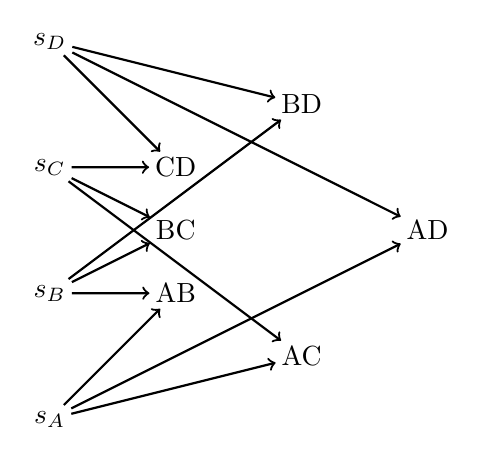
\begin{tikzpicture}[scale=0.8,help lines/.style={color=lightgray,line 
width=0.2pt},post/.style={->,shorten >=1pt,>=stealth',thick}]
    
    \node[inner sep=2] (sa) at (0.0,2.0) {$s_A$};
    \node[inner sep=2] (sb) at (0.0,4.0) {$s_B$};
    \node[inner sep=2] (sc) at (0.0,6.0) {$s_C$};
    \node[inner sep=2] (sd) at (0.0,8.0) {$s_D$};

    \node[inner sep=2] (AB) at (2.0,4.0) {AB};
    \node[inner sep=2] (BC) at (2.0,5.0) {BC};
    \node[inner sep=2] (CD) at (2.0,6.0) {CD};

    \node[inner sep=2] (AC) at (4.0,3.0) {AC};
    \node[inner sep=2] (BD) at (4.0,7.0) {BD};

    \node[inner sep=2] (AD) at (6.0,5.0) {AD};

    \draw[->, thick] (sa) -- (AB);
    \draw[->, thick] (sa) -- (AC);
    \draw[->, thick] (sa) -- (AD);

    \draw[->, thick] (sb) -- (BC);
    \draw[->, thick] (sb) -- (BD);
    \draw[->, thick] (sb) -- (AB);

    \draw[->, thick] (sc) -- (AC);
    \draw[->, thick] (sc) -- (BC);
    \draw[->, thick] (sc) -- (CD);

    \draw[->, thick] (sd) -- (AD);
    \draw[->, thick] (sd) -- (CD);
    \draw[->, thick] (sd) -- (BD);
    
    \end{tikzpicture}
    \caption{Belief network}
    \label{fig:BinGame_DAG}    
\end{figure}

The skill levels of the players \emph{a posteriori} are not independent, because
the games' results are colliders between the skill levels. Consequently, after
conditioning on the outcomes, they are dependent. This makes intuitive sense: if
one has observed that A often beats B, one's beliefs about A's skill are now related to
one's beliefs about B's skill.

The probability that D will beat A is obtained by inference, using Bayes' rule: $p(\mathbf{s} \; | \;
results) = \frac{p(results \; | \; \mathbf{s}) p(\mathbf{s})}{p(results)}$, where
$p(result = X \; defeats \; Y \; | \; \mathbf{s}) = \frac{1}{1 + \exp{s_y - s_x}}$. Using the
given results, we infer a posterior distribution for $\mathbf{s}$. In turn, we use this posterior
distribution to calculate a probability for $p(result = D \; defeats \; A \; | \;
\mathbf{s}) p(\mathbf{s})$. This probability is calculated to be $0.0143$.

Using the same inferred distribution for $p(\mathbf{s} \; | \; results)$, we
evaluate the expectation of each element of $\mathbf{s}$, according to
$\langle s_i \rangle = \sum_{s_i} s_i p(s_i \; | \; s_{j \neq i})$.
These expectations are found to be as follows:

\begin{equation}
s_A  = 8.3 \; s_B = 5.5 \; s_C = 6.7 \; s_D = 2.2
\end{equation}

The code used to estimate these probabilities is given in the listings below.

\begin{lstlisting}
clear all;

p_s = 1/10 * ones(10,10,10,10);


results = [ 1 -1  0  0; ...
            1 -1  0  0; ...
            0  1 -1  0; ...
            0  1 -1  0; ...
            1  0 -1  0; ...
            1  0 -1  0; ...
           -1  0  1  0; ...
            0  0  1 -1; ...
            0  0  1 -1 ];
        
for i=1:length(results)
    [p_s, ~] = update_s(results(i,:), p_s);
end

new_results = [-1 0 0 1];
[~, p_result_on_s] = update_s(new_results, p_s);

p_DbA = 0;

for i=1:10
    for j=1:10
        p_DbA = p_DbA + p_result_on_s(i,j) .* sum(sum(p_s(j,:,:,i)));
    end
end


A = squeeze(sum(sum(sum(p_s, 3), 2), 4));
B = squeeze(sum(sum(sum(p_s, 3), 1), 4))';
C = squeeze(sum(sum(sum(p_s, 2), 1), 4));
D = squeeze(sum(sum(sum(p_s, 2), 1), 3));

vec = 1:10;

means = [vec*A; vec*B; vec*C; vec*D]
\end{lstlisting}


\begin{lstlisting}
function [p_s_on_result, p_result_on_s] = update_s(result, s_prior_matrix)
    winner = find(result==1);
    loser = find(result==-1);
    possible_s = 1:1:10;

    for i_win=1:10
        for j_lose=1:10
            p_result_on_s(i_win,j_lose) = 1/(1+exp(possible_s(j_lose)-possible_s(i_win)));
        end
    end
    
    p_s_w_by_l = zeros(10,10,10,10);
    
    for i=1:10
        for j=1:10
            % TODO: reimplement this using metaprogramming, e.g. in Julia
            if winner==1 && loser==2
                p_s_w_by_l(i,j,:,:) = p_result_on_s .* squeeze(s_prior_matrix(i,j,:,:));

            elseif winner==1 && loser==3
                p_s_w_by_l(i,:,j,:) = p_result_on_s .* squeeze(s_prior_matrix(i,:,j,:));
                
            elseif winner==1 && loser==4
                p_s_w_by_l(i,:,:,j) = p_result_on_s .* squeeze(s_prior_matrix(i,:,:,j));
                
            elseif winner==2 && loser==1
                p_s_w_by_l(j,i,:,:) = p_result_on_s .* squeeze(s_prior_matrix(j,i,:,:));
                
            elseif winner==2 && loser==3
                p_s_w_by_l(:,i,j,:) = p_result_on_s .* squeeze(s_prior_matrix(:,i,j,:));
                
            elseif winner==2 && loser==4
                p_s_w_by_l(:,i,:,j) = p_result_on_s .* squeeze(s_prior_matrix(:,i,:,j));
                
            elseif winner==3 && loser==1
                p_s_w_by_l(j,:,i,:) = p_result_on_s .* squeeze(s_prior_matrix(j,:,i,:));
                
            elseif winner==3 && loser==2
                p_s_w_by_l(:,j,i,:) = p_result_on_s .* squeeze(s_prior_matrix(:,j,i,:));
                
            elseif winner==3 && loser==4
                p_s_w_by_l(:,:,i,j) = p_result_on_s .* squeeze(s_prior_matrix(:,:,i,j));
                
            elseif winner==4 && loser==1
                p_s_w_by_l(j,:,:,i) = p_result_on_s .* squeeze(s_prior_matrix(j,:,:,i));
                
            elseif winner==4 && loser==2
                p_s_w_by_l(:,j,:,i) = p_result_on_s .* squeeze(s_prior_matrix(:,j,:,i));
                
            elseif winner==4 && loser==3
                p_s_w_by_l(:,:,j,i) = p_result_on_s .* squeeze(s_prior_matrix(:,:,j,i));
                
            end
        end
    end
    
    p_s_on_result = p_s_w_by_l / sum(sum(sum(sum(p_s_w_by_l))));
end

\end{lstlisting}

\section*{Problem 3.22}

We model this problem with a Bayesian network described as:

$$p(d, s_A, s_B, s_C) = p(d | s_A, s_B, s_C) p(s_A, s_B, s_C)$$ having the 
following graph: 

\begin{figure}[H]
  \centering
    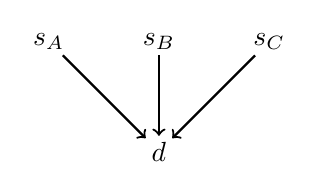
\begin{tikzpicture}[scale=01.4,help lines/.style={color=lightgray,line 
width=0.2pt},post/.style={->,shorten >=1pt,>=stealth',thick}]
    
    \node[inner sep=2] (sa) at (-1.0,0.0) {$s_A$};
    \node[inner sep=2] (sb) at (0.0,0.0) {$s_B$};
    \node[inner sep=2] (sc) at (1.0,0.0) {$s_C$};
    \node[inner sep=2] (d) at (0.0,-1.0) {$d$};

    \draw[->, thick] (sa) -- (d);
    \draw[->, thick] (sb) -- (d);
    \draw[->, thick] (sc) -- (d);
    
    \end{tikzpicture}
    \caption{Avertisement Bayesian network}
    \label{fig:daily_fail}    
\end{figure}

For each data entry $(a_i, a_j, a_k)$, we first calculate the joint probability
$$p(d = a_i, s_A, s_B, s_C) = p(d = a_i | s_A, s_B, s_C)p(s_A, s_B, s_C)$$. 
This will then be marginalised to get: 
$$ p(d = a_i, s_A) = \sum_{BC}p(d = a_i, s_A, s_B, s_C) $$
$$ p(d = a_i, s_B) = \sum_{BC}p(d = a_i, s_A, s_B, s_C) $$
$$ p(d = a_i, s_C) = \sum_{BC}p(d = a_i, s_A, s_B, s_C) $$

The probability $p(d = a_i, s_A)$ is then normalised and used for updating the 
probability $p(s_A)$:
$$p(s_A) = p(s_A)p(d = a_i, s_A)$$
The other probabilities $p(s_B)$ and $p(s_C)$ are updated in a similar fashion. 

At the end, the expected interest is calculated using the formula

$$E[s_A] = \sum_{i=1}^{5}i\ * p(s_A)$$

The final interest levels we get are:
$$\left[\; 3.5103, 1.3489, 1.0755, 2.3107, 1.4150, 4.5783, 1.6438, 4.5783, 
4.4519, 3.5103\; \right]$$

The MATLAB code that was used to calculate them is:
% TODO: make the MATLAB code calculate the joint distribution and 
%then marginalise

\begin{lstlisting}
 function [] = prob322()

data = [1 2 3; 2 5 3; 4 7 10; 6 3 4; 6 8 5; 9 3 7; 10 2 4; 7 1 2; 8 7 2; 8 3 6; 
8 6 4; 4 3 9; 5 4 1; 9 5 1; 6 7 8; 4 9 7; 10 8 6; 5 4 3; 6 3 2; 1 4 2];

nrDataPoints = 10;
nrLevels = 5;
interest_adv = ones(nrDataPoints, nrLevels) .* 0.2;

pDgABC = zeros(nrLevels, nrLevels, nrLevels);

for sA = 1:nrLevels
    for sB = 1:nrLevels
        for sC = 1:nrLevels
            pDgABC(sA, sB, sC) = exp(sA - max(sB, sC));
        end
    end
end

% calculate the marginal p(sA)
pSa = zeros(1, nrLevels);
for sA = 1:nrLevels
    pSa(sA) = sum(sum(pDgABC(sA, :, :)));
end

% calculate the marginal p(Sb). Note that p(Sc) = p(Sb)
pSb = zeros(1, nrLevels);
for sB = 1:nrLevels
    pSb(sB) = sum(sum(pDgABC(:, sB, :)));
end

% normalise the values (not strictly needed though)
pSa = pSa ./ sum(pSa);
pSb = pSb ./ sum(pSb);

for i=1:nrDataPoints
    dataPoint = data(i,:);
    
    advA = dataPoint(1);
    advB = dataPoint(2);
    advC = dataPoint(3);
    
    interest_adv(advA,:) = interest_adv(advA,:) .* pSa;
    interest_adv(advB,:) = interest_adv(advB,:) .* pSb;
    interest_adv(advC,:) = interest_adv(advC,:) .* pSb; % using pSb since pSc = 
pSb
    
    interest_adv(advA,:) = interest_adv(advA,:) ./ sum(interest_adv(advA,:));
    interest_adv(advB,:) = interest_adv(advB,:) ./ sum(interest_adv(advB,:));
    interest_adv(advC,:) = interest_adv(advC,:) ./ sum(interest_adv(advC,:));
    % calc prob(sA)

end

expected_values = zeros(nrDataPoints,1);
for level=1:nrLevels
    expected_values = expected_values + interest_adv(:,level) * level;
end

expected_values
end
\end{lstlisting}


\section*{Extra Problem A}

The image cleaning algorithm given here relies upon striking a balance between
the first term, which tries to encourage similarity of pixel values in a small
neighbourhood; and the second term, which tries to encourage similarity
(somewhat) to the noisy image. 

Numerical solution, to optimise $x$, is implemented by random perturbation of
$x$ at each step. These perturbations are only accepted if they
increase/decrease \hilight{Raz: choose increase/decrease as appropriate, and
put in details of the converged equilibrium, code listings and the image.} the objective functions, however, which for this problem
eventually leads to a solution.

The algorithm is actually meant to maximise the objective function given in the 
assignment specification. Our implementation randomly selects a pixel to get 
updated, calculates the objective function of the original image and the new 
image (having the pixel swapped) and decides to update the pixel value if the 
value of the objection function is higher. After running for 1,320,000 
iterations, our algorithm gives the following image: 



\begin{figure}[H]
  \centering
  \begin{subfigure}[b]{0.3\textwidth}
	  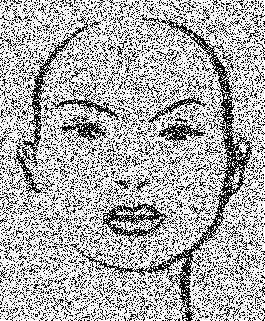
\includegraphics[scale=0.6]{plots/xnoisy}
	  \caption{Original image}
	  \label{fig:gull}
  \end{subfigure}%
  ~ 
  \begin{subfigure}[b]{0.3\textwidth}
	  
\includegraphics[scale=0.6]{plots/xclean0132}
	  \caption{Final image}
	  \label{fig:tiger}
  \end{subfigure}
%   \caption{Pictures of animals}\label{fig:animals}
\end{figure}

The MATLAB code that was used to run this program is given below:

\begin{lstlisting}
function xclean = extra1()

load('noisyface.mat')

[h w] = size(xnoisy);

nrPixels = w * h;

xclean = xnoisy;

noChangeTimes = 0;
iteration = 1;
module_size = 10000;
    
while (noChangeTimes < 5 * nrPixels)

    % get me a random pixel to update
    nextPixelI = floor(rand * h) + 1;
    nextPixelJ = floor(rand * w) + 1;

    % clone the image file and flip the pixel
    flipped_pixel_img = xclean;
    flipped_pixel_img(nextPixelI, nextPixelJ) = 1 - 
flipped_pixel_img(nextPixelI, nextPixelJ);

    % calculate the objective functions
    valUnchanged = objective_func(xclean, xnoisy);
    valFlipped = objective_func(flipped_pixel_img, xnoisy);

    % compare the values of the objective function and update if necessary
    if(valFlipped > valUnchanged)
       % pixel was flipped 
       xclean = flipped_pixel_img;
       noChangeTimes = 0;
    else
       % pixel not flipped
       noChangeTimes = noChangeTimes + 1;
    end


    if(mod(iteration,module_size) == 0)
        iteration
        noChangeTimes
        index =  sprintf('%04d', iteration / module_size)
        imwrite(xclean,strcat('images/xclean', index,  '.png'));
    end
    iteration = iteration + 1;
    
end


end

function val = objective_func(image, original_noisy)

val = 0;
neigh_w = 10;

% create copies of the original image slided to the right and down
right_slided = image(:,2:end);
down_slided = image(2:end,:);

% chop 1 row/column of the original image and create copies
right_chopped = image(:,1:end-1);
down_chopped = image(1:end-1,:);

% compate the chopped version with the slided ones
right_eq = right_slided == right_chopped;
down_eq = down_slided == down_chopped;

% calculate the value of the objective function
val =  val + neigh_w  * 2 * (sum(sum(right_eq)) + sum(sum(down_eq)));
val = val + 2 * sum(sum(original_noisy .* image));


end
\end{lstlisting}


\section*{Extra Problem B}


\end{document}
